\subsection{Geração de Código}
\emph{Geração de Código} é o processo de utilizar todas as informações
geradas durante as fases de \emph{análise} (Léxica, Sintática etc) para
gerar o programa-objeto. Conforme a arquitetura do compilador, é possível
incluir outras etapas intermediárias, conhecidas como \emph{Representações
Intermediárias} (RI), que visam possibilitar otimizações no programa-objeto
gerado \cite{louden97-pt}.

Uma forma possível de RI é conhecida com \emph{código-de-três-endereços}. Este
formato é conhecido desta forma pois possui a seguinte forma de instruções $x
= y \textbf{op} z$, ou seja, do lado direito da atribuição possui apenas um
operador binário, seus operandos e do lado esquerdo a variável que armazena o
resultado da operação. Variações são permitidas para representar, por exemplo,
o sinal de menos unário $x = -y$.

\begin{lstlisting}[label=lst:three_addresses,caption=Código de 3 Endereços]
t1 = c * d
t2 = a + b
t3 = t1 + t2
x = t3
\end{lstlisting}

A Listagem \ref{lst:three_addresses} demonstra um exemplo do
código-de-três-endereços para a expressão $x=a+b+c*d$. As variáveis
$\text{t}i$ para $i \in \{1,2,3\}$ representam variáveis temporárias criadas pelo próprio
compilador.

Para este projeto, não são geradas RIs, apenas os programas-objeto em
\emph{Linguagem C}, que posteriormente podem ser compiladas por um compilador
C, como o \emph{gcc}, gerando um programa executável, e em \emph{Linguagem
DOT} possibilitando a geração de uma representação gráfica do programa.
Mais referências sobre RIs e códigos-de-três-endereços são encontradas em
\citeonline{new-dragon-pt} e \citeonline{louden97-pt}.

Conforme exposto, este projeto de compilador atua como um tradutor entre
linguagens. Uma abordagem semelhante foi utilizada na implementação inicial da
\emph{Linguagem C++}. Este compilador traduzia programas C++ para programas C
para que pudessem, posteriormente, ser compilados por um compilador C
disponível. Assim, podemos considerar o processo de compilação como um
processo de tradução de uma linguagem de nível mais alto para uma outra
linguagem de nível mais baixo, repetindo o  processo até que seja produzido um
programa executável na máquina-alvo \cite{new-dragon-pt}.

A Geração de Código também consiste num processo de linearização das
estruturas de árvores disponibilizadas pelas fases anteriores, transformando,
por exemplo, uma árvore sintática em um programa C, em que as instruções são
escritas linearmente em um arquivo.

A Listagem \ref{lst:code_gen} demonstra uma possível implementação, em
pseudo-código, de função geradora de código, tendo como base uma árvore
sintática em que cada nó possui até dois filhos. Notamos que a função pode
vistar a árvore em pré-ordem, em ordem e pós-ordem.

\begin{lstlisting}[label=lst:code_gen,caption=Exemplo Gerador de Código]
funcao geraCodigo (no_arvore T)
inicio
	gerar_codigo_preparatorio(T)
	gerar_codigo(T)
	gerar_codigo_preparatorio_filho_esquerda(T->filho_esquerda)
	gerar_codigo_filho_esquerda(T->filho_esquerda)
	gerar_codigo_preparatorio_filho_direita(T->filho_direita)
	gerar_codigo_filho_direita(T->filho_direita)
	gerar_codigo_final(T)
fim
\end{lstlisting}

Com pequenas alterações no código da Listagem \ref{lst:code_gen}, podemos
incluir mais filhos aos nós filhos à árvore $T$, bem como, representar a
construção de quase todas as contruções necessárias para produzir o
programa-objeto.


\subsubsection{Linguagem DOT}
\label{sec:impl_gen_dot}

Segundo \citeonline{EGKNW03}:

\begin{citacao}{4cm}{0cm}
Graphviz is a collection of software for viewing and manipulating abstract
graphs. It provides graph visualization for tools and web sites in domains
such as software engineering, networking, databases, knowledge representation,
and bio-informatics
\end{citacao}

Um dos softwares dessa coleção é o compilador \emph{dot}. Segundo
\citeonline{gansner09}:

\begin{citacao}{4cm}{0cm}
\textbf{dot} draws directed graphs. It reads attributed graph text files and
writes drawings, either as graph files or in a graphics format such as GIF,
PNG, SVG, PDF, or PostScript.
\end{citacao}

\textbf{dot} aceita como entrada um arquivo de texto expresso na Linguagem
DOT (verificar \url{http://graphviz.org/content/dot-language}). Essa
linguagem define três tipos principais de objetos: grafos, nós e arestas.
O grafo principal (mais externo) pode ser direcionado (\emph{digraph} {--}
\emph{directed graph}, ou seja, grafo direcionado), ou não-direcionado. Em um
grafo principal, é possivel termos um sub-grafo (\emph{subgraph}) que permite
a definições de nós e arestas \cite{gansner09}.

Um nó é criado quando o seu nome aparece pela primeira vez no arquivo. As
arestas são criadas quando dois nós são ligados pelo operador de aresta {->}.

Na Listagem \ref{lst:dot_example} temos o exemplo de um grafo escrito em
DOT que após sua compilação com o comando
$$
\text{dot} \quad \text{-Tpng} \quad \text{exemplo\_dot.gv} \quad \text{>}
\quad \text{exemplo\_dot.png}
$$
gerará a representação gráfica demonstrada na Figura \ref{fig:dot_example}.

\lstinputlisting[label=lst:dot_example, caption=Exemplo de Grafo Expresso em DOT]{src_files/dot_example.gv}

\begin{figure}
	\begin{center}
		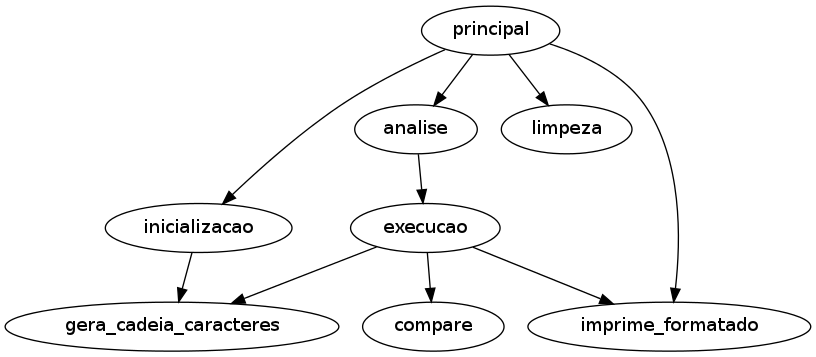
\includegraphics[scale=0.4]{dot_example}
	\end{center}
	\caption{Exemplo Grafo Gerado pelo dot}
	\label{fig:dot_example}
\end{figure}
